\chapter{EDA on Bearings Dataset}
\label{sec:bearings-eda}


\section{Introduction to EDA Chapter}

In this chapter, we discuss \ac{eda}, an indispensable step in data analysis. \ac{eda} focuses on gaining a comprehensive understanding of the data using descriptive statistics and graphical methods before the application of sophisticated statistical techniques or machine learning algorithms.

The purpose of our EDA is to delve into a dataset that includes measurements related to the performance of shaft bearings. These measurements include \(Fr\) (radial force), \(n\) (rotational speed), and \(Lifetime\) (expected bearing lifetime). Through our \ac{eda}, we aim to understand the distributions of these variables and their interactions.

Such insights derived from \ac{eda} can be valuable for further data processing, hypothesis testing, feature selection, and machine learning model selection. In our specific context, understanding the factors that affect the lifetime of a bearing can help make informed decisions related to their operation and maintenance.

Our EDA process will be systematic and iterative, revising our understanding as new insights emerge. We will walk through an initial data inspection, followed by univariate and multivariate analyses, ultimately leading to feature engineering and hypothesis generation.


\section{Initial Data Inspection}

The first step in our \ac{eda} is the initial inspection of the dataset. This involves loading the data, examining a few records, identifying the type of each variable, checking for missing values, and noting the range of values each variable can take. A selection of data points from the dataset is presented in Table \ref{table:bearings-dataset} for initial observation.

\begin{table}[ht]
  \centering
  \caption{Sample of the Dataset}
  \label{table:bearings-dataset}
  \begin{tabular}{|c|c|c|c|}
  \hline
  Line & Fr & n & Lifetime \\
  \hline
  1 & 200 & 100 & 88,445,568.46 \\
  2 & 200 & 200 & 44,222,784.23 \\
  ... & ... & ... & ... \\
  34 & 200 & 3400 & 2,601,340.249 \\
  35 & 200 & 3500 & 2,527,016.242 \\
  36 & 300 & 100 & 22,893,132.09 \\
  37 & 300 & 200 & 11,446,566.04 \\
  ... & ... & ... & ... \\
  69 & 300 & 3400 & 673,327.4144 \\
  70 & 300 & 3500 & 654,089.4882 \\
  71 & 400 & 100 & 8,774,911.776 \\
  72 & 400 & 200 & 4,387,455.888 \\
  ... & ... & ... & ... \\
  1364 & 4000 & 3400 & 119.7927427 \\
  1365 & 4000 & 3500 & 116.3700929 \\
  \hline
  \end{tabular}
\end{table}

Our dataset is a structured one, with \(Fr\) and \(n\) recorded as integer values and \(Lifetime\) as a floating-point number. \(Fr\) represents the radial force applied on the bearing in Newton (N) and ranges from 200 to 4000 N. \(n\) represents the rotational speed in rotations per minute (rpm) and spans values from 100 to 3500 rpm. \(Lifetime\) is the expected lifetime of the bearing in hours (h) and varies from 88,445,568.46 h to 116.37 h. A significant observation made at this point is the step-wise increment pattern seen in \(Fr\) and \(n\), and the corresponding decrement in \(Lifetime\). Each unique combination of \(Fr\) and \(n\) represents different operational conditions for the bearing, and their influence on the bearing's expected \(Lifetime\) is our primary point of interest.

No missing values are present in the dataset, which allows us to proceed with the analysis without the need for imputation or deletion strategies.


\section{Univariate Analysis}

Univariate analysis provides deeper insight into each feature independently. Its primary goal is to examine the distribution of each feature, detect potential outliers, and determine whether any transformations might be necessary.

As previously noted, the \(Fr\) and \(n\) variables show a structured, uniform distribution due to the step-wise pattern of data recording. This setup ensures a comprehensive coverage of various operational conditions.

The main focus of our univariate analysis is on the \(Lifetime\) variable. A notable observation is that \(Lifetime\) follows an exponential decrease pattern as \(Fr\) and \(n\) increase. This behavior suggests a potential non-linear relationship between \(Lifetime\) and the operational parameters \(Fr\) and \(n\).

To better visualize the distribution of \(Lifetime\), we employed histograms and boxplots (Figure \ref{fig:bearings-histogram} and Figure \ref{fig:bearings-boxplot}). Since \(Lifetime\) features a long tail towards lower values, we transformed the data using a log function. This transformation helped us to bucket the \(Lifetime\) data into more meaningful intervals for visualization, revealing a clearer distribution pattern.

\begin{figure}[ht]
    \centering
    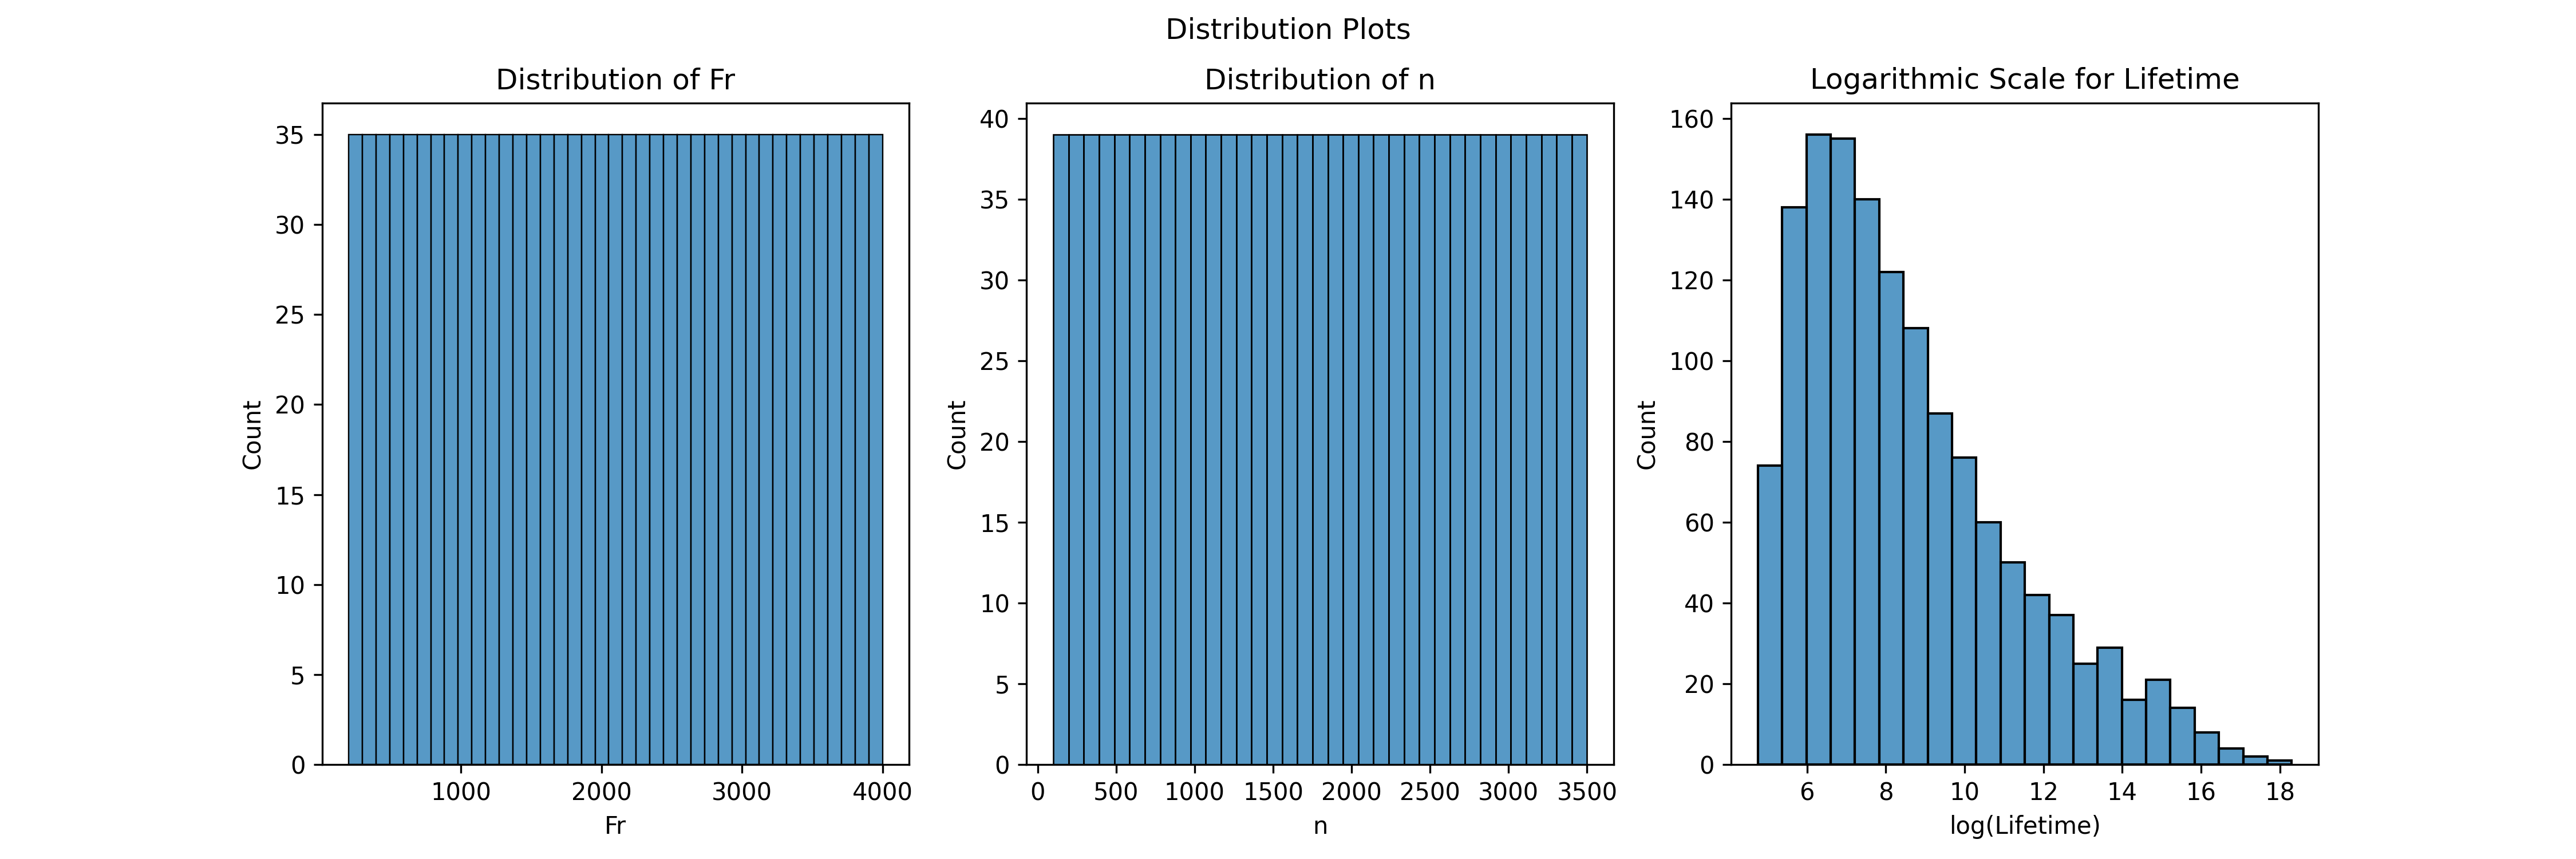
\includegraphics[width=\textwidth]{assets/bearings-eda/histogram.png}
    \caption{Histogram of Lifetime}
    \label{fig:bearings-histogram}
\end{figure}

\begin{figure}[ht]
    \centering
    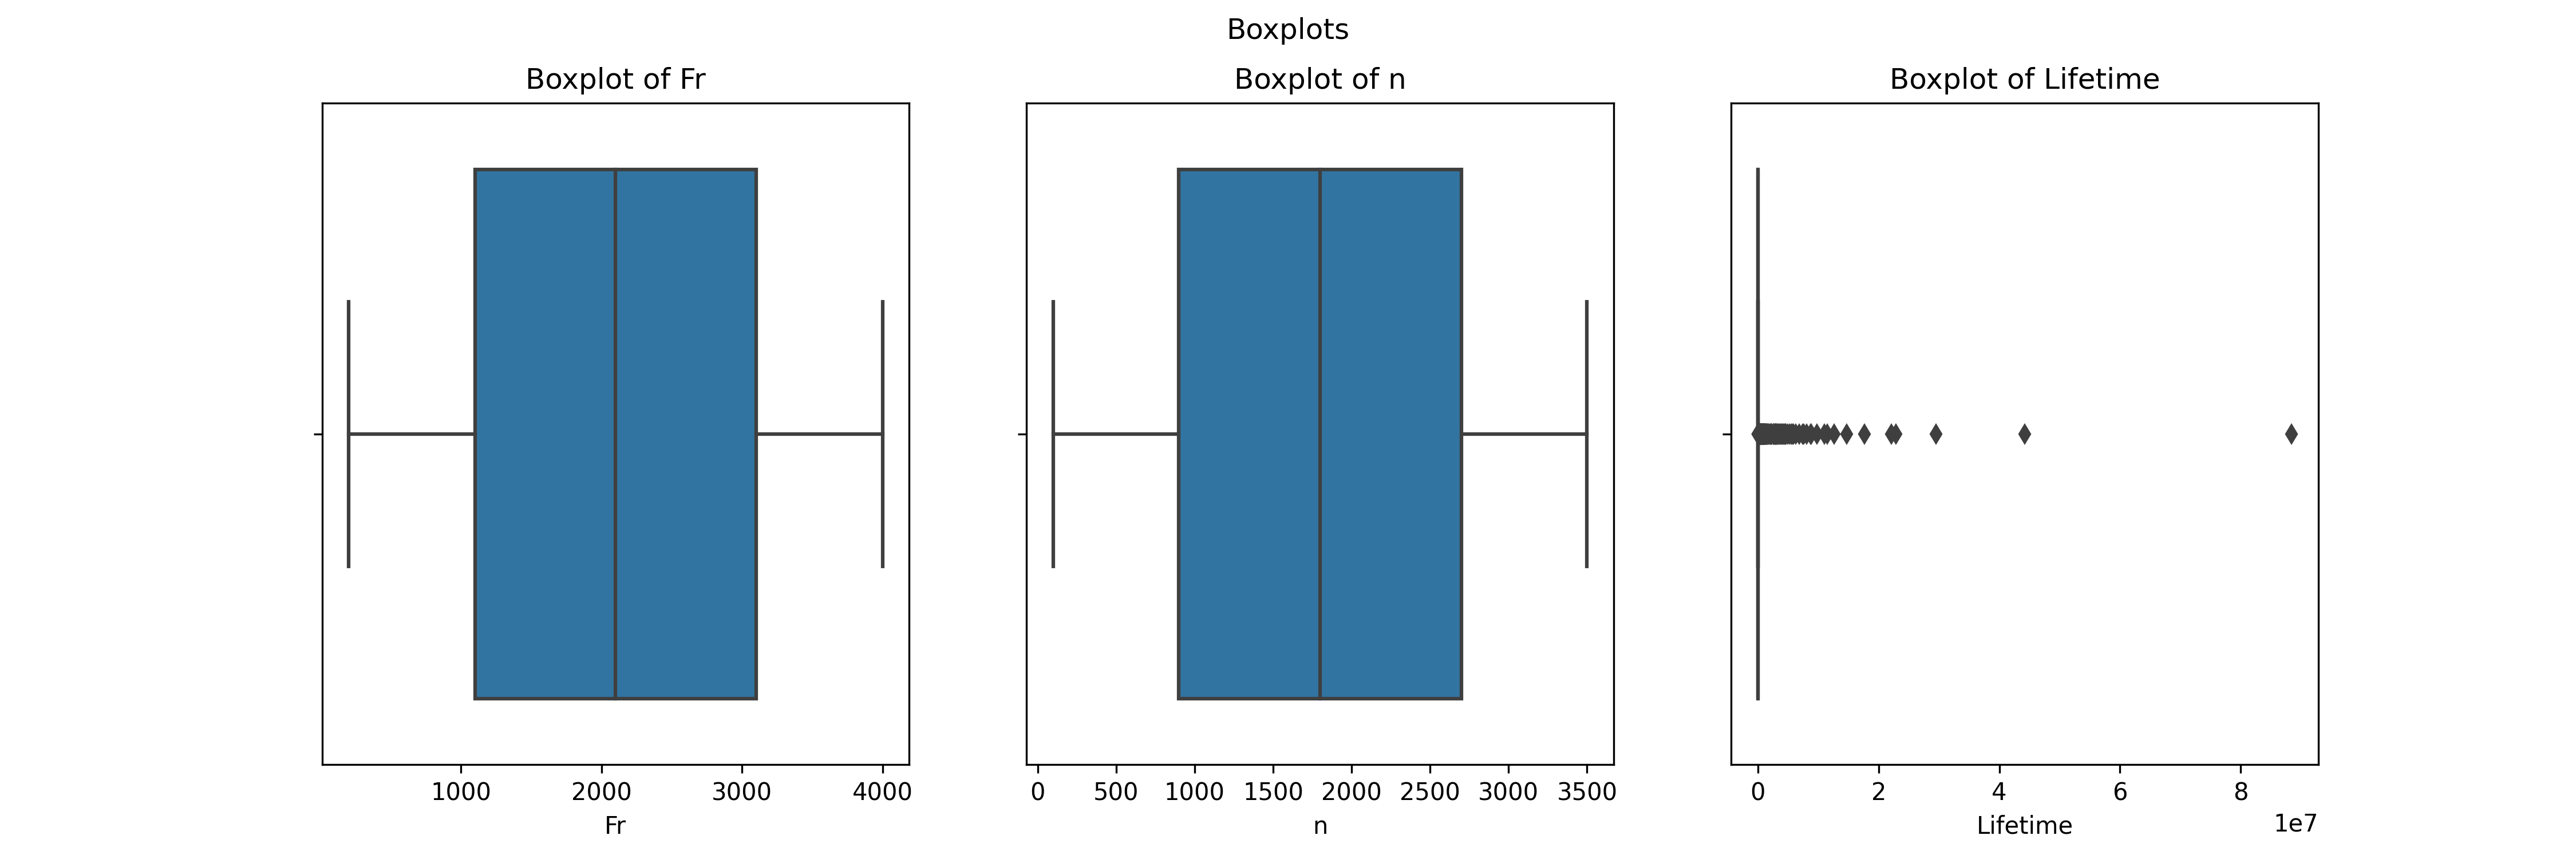
\includegraphics[width=\textwidth]{assets/bearings-eda/boxplot.png}
    \caption{Boxplot of Lifetime}
    \label{fig:bearings-boxplot}
\end{figure}

While the \(Lifetime\) data features a wide range of values, this is to be expected given the nature of the measured attribute. The variation can be attributed to the range of operating conditions (\(Fr\) and \(n\)) represented in the dataset. In this context, extreme values in \(Lifetime\) are not necessarily outliers in the traditional sense, but rather indicate the broad spectrum of potential lifetimes for the shaft bearings under different conditions.

Overall, univariate analysis offers valuable insights into each feature's characteristics. It also paves the way for a more nuanced understanding of interactions between features in the subsequent multivariate analysis.


\section{Multivariate Analysis}

In the process of \ac{eda}, multivariate analysis plays a critical role in examining the interrelationships between different features. Simultaneously, the insights gleaned during this process can inform the creation of new features, enhancing our dataset and offering further explanatory power for our hypotheses.

To understand the relationships between the variables \(Fr\), \(n\), and \(Lifetime\), we used various visualization techniques, including 3D plots, pair plots, and correlation matrices.

A 3D plot, representing the three variables, allowed us to perceive the nature of the interactions between them. We observed a significant decrease in \(Lifetime\) with an increase in either \(Fr\) or \(n\). This trend is indicative of an inverse exponential relationship between these variables. The relationship was more pronounced with \(Fr\), implying that \(Fr\) had a greater impact on the \(Lifetime\) compared to \(n\).

\begin{figure}[ht]
    \centering
    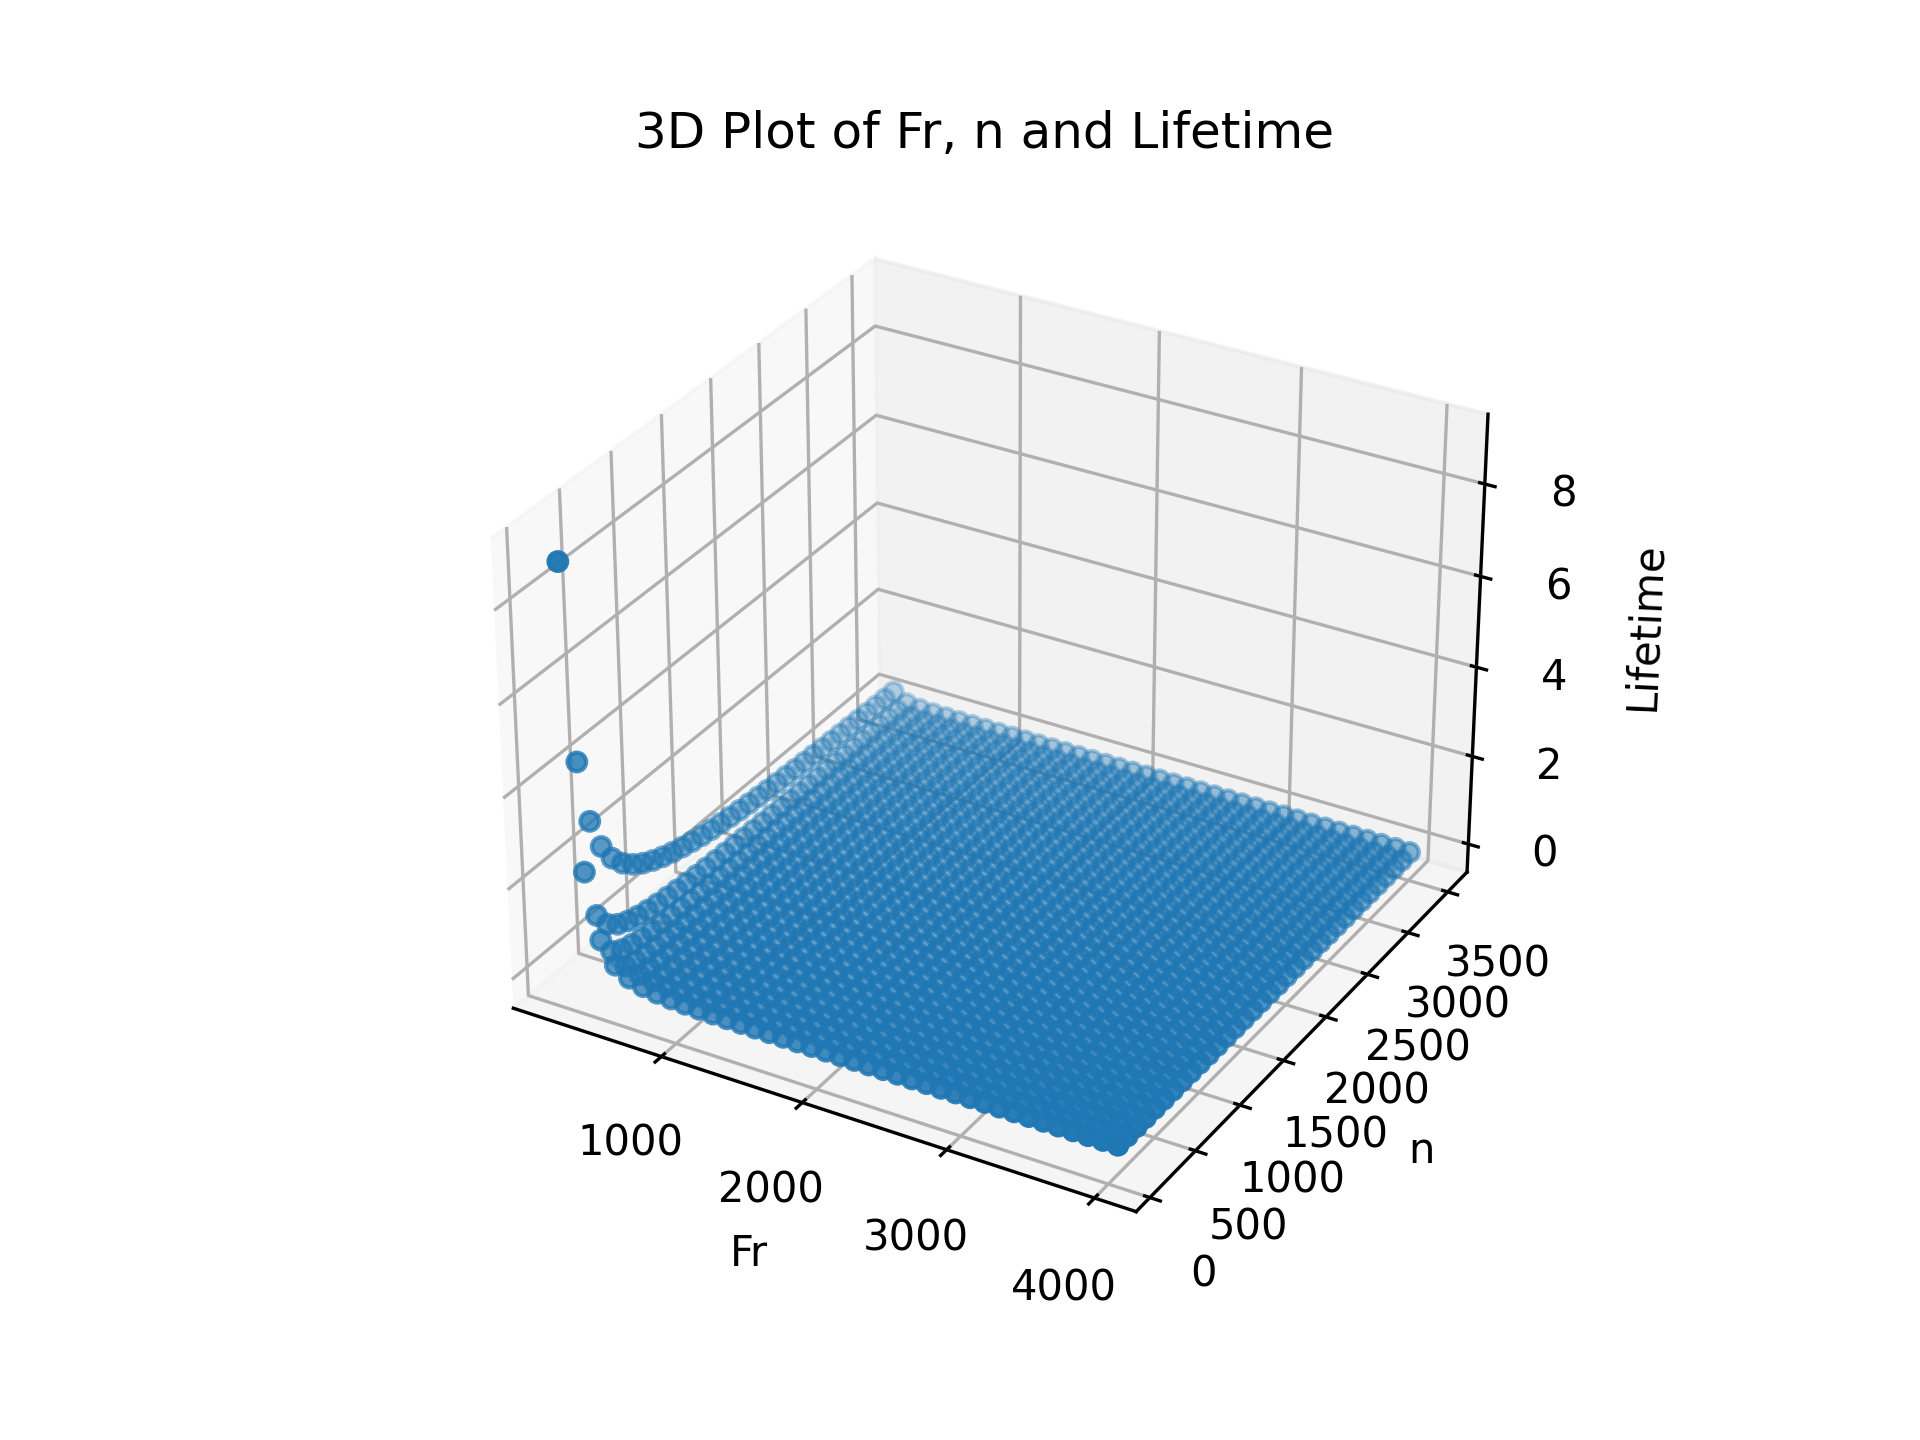
\includegraphics[width=\textwidth]{assets/bearings-eda/3dplot.png}
    \caption{3D plot of Fr, n, and Lifetime}
    \label{fig:bearings-3dplot}
\end{figure}

Recognizing the potential exponential relationship, we engineered two new features, \(Fr \cdot n\) and \(Fr/n\), to further investigate these relationships. The choice of these features was motivated by their ability to reveal the interactions and the relative impact of \(Fr\) and \(n\) on \(Lifetime\).

Subsequently, pair plots and correlation matrices (Figures \ref{fig:bearings-pairplot} and \ref{fig:bearings-corrmat}) were generated, incorporating the original and engineered features. These visualizations provided insights into the relationships and correlations between the variables, aiding in the derivation of the exponent in our hypothesis equation.

\begin{figure}[ht]
    \centering
    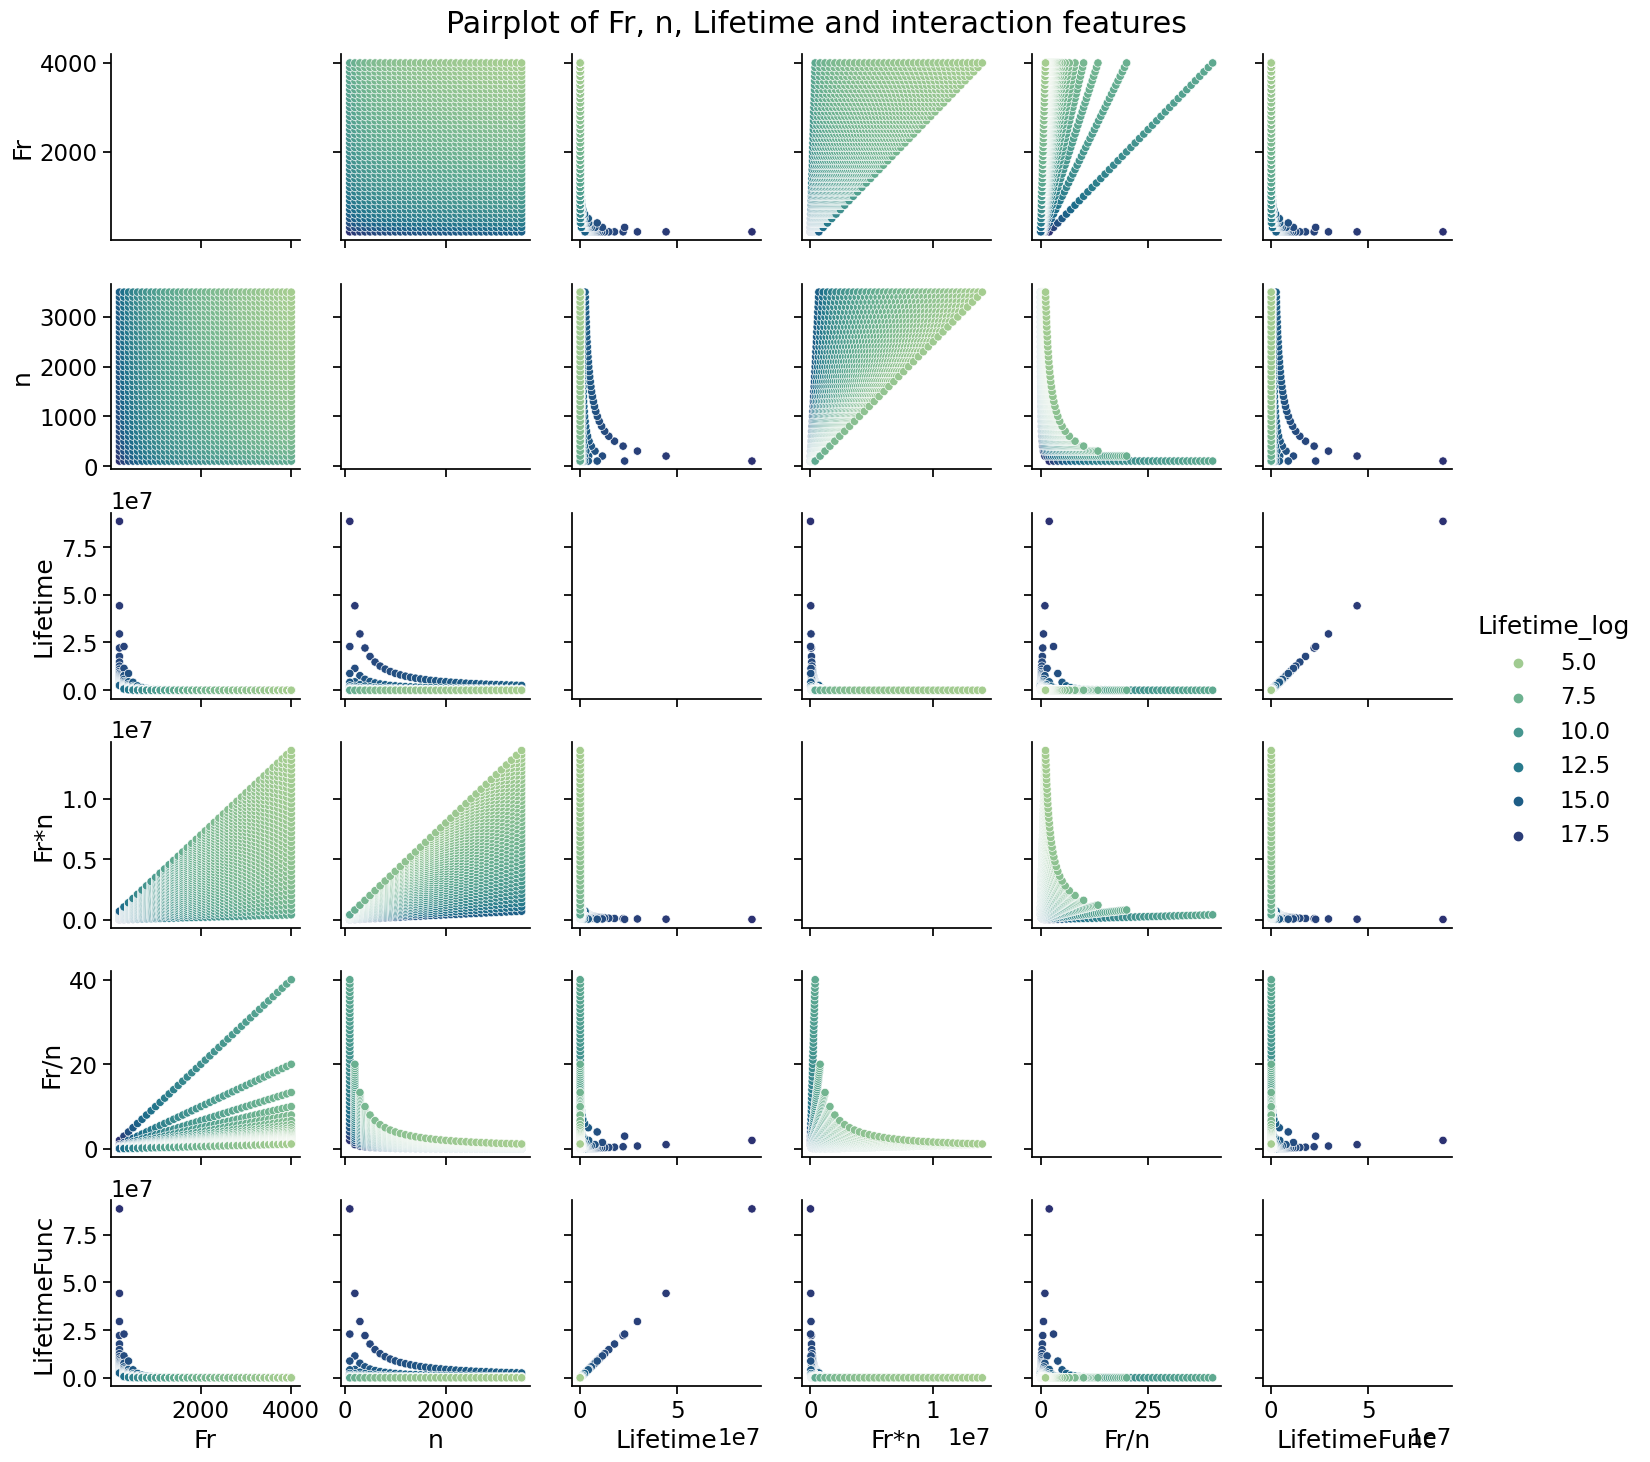
\includegraphics[width=\textwidth]{assets/bearings-eda/pairplot.png}
    \caption{Pairplot of variables}
    \label{fig:bearings-pairplot}
\end{figure}

\begin{figure}[ht]
    \centering
    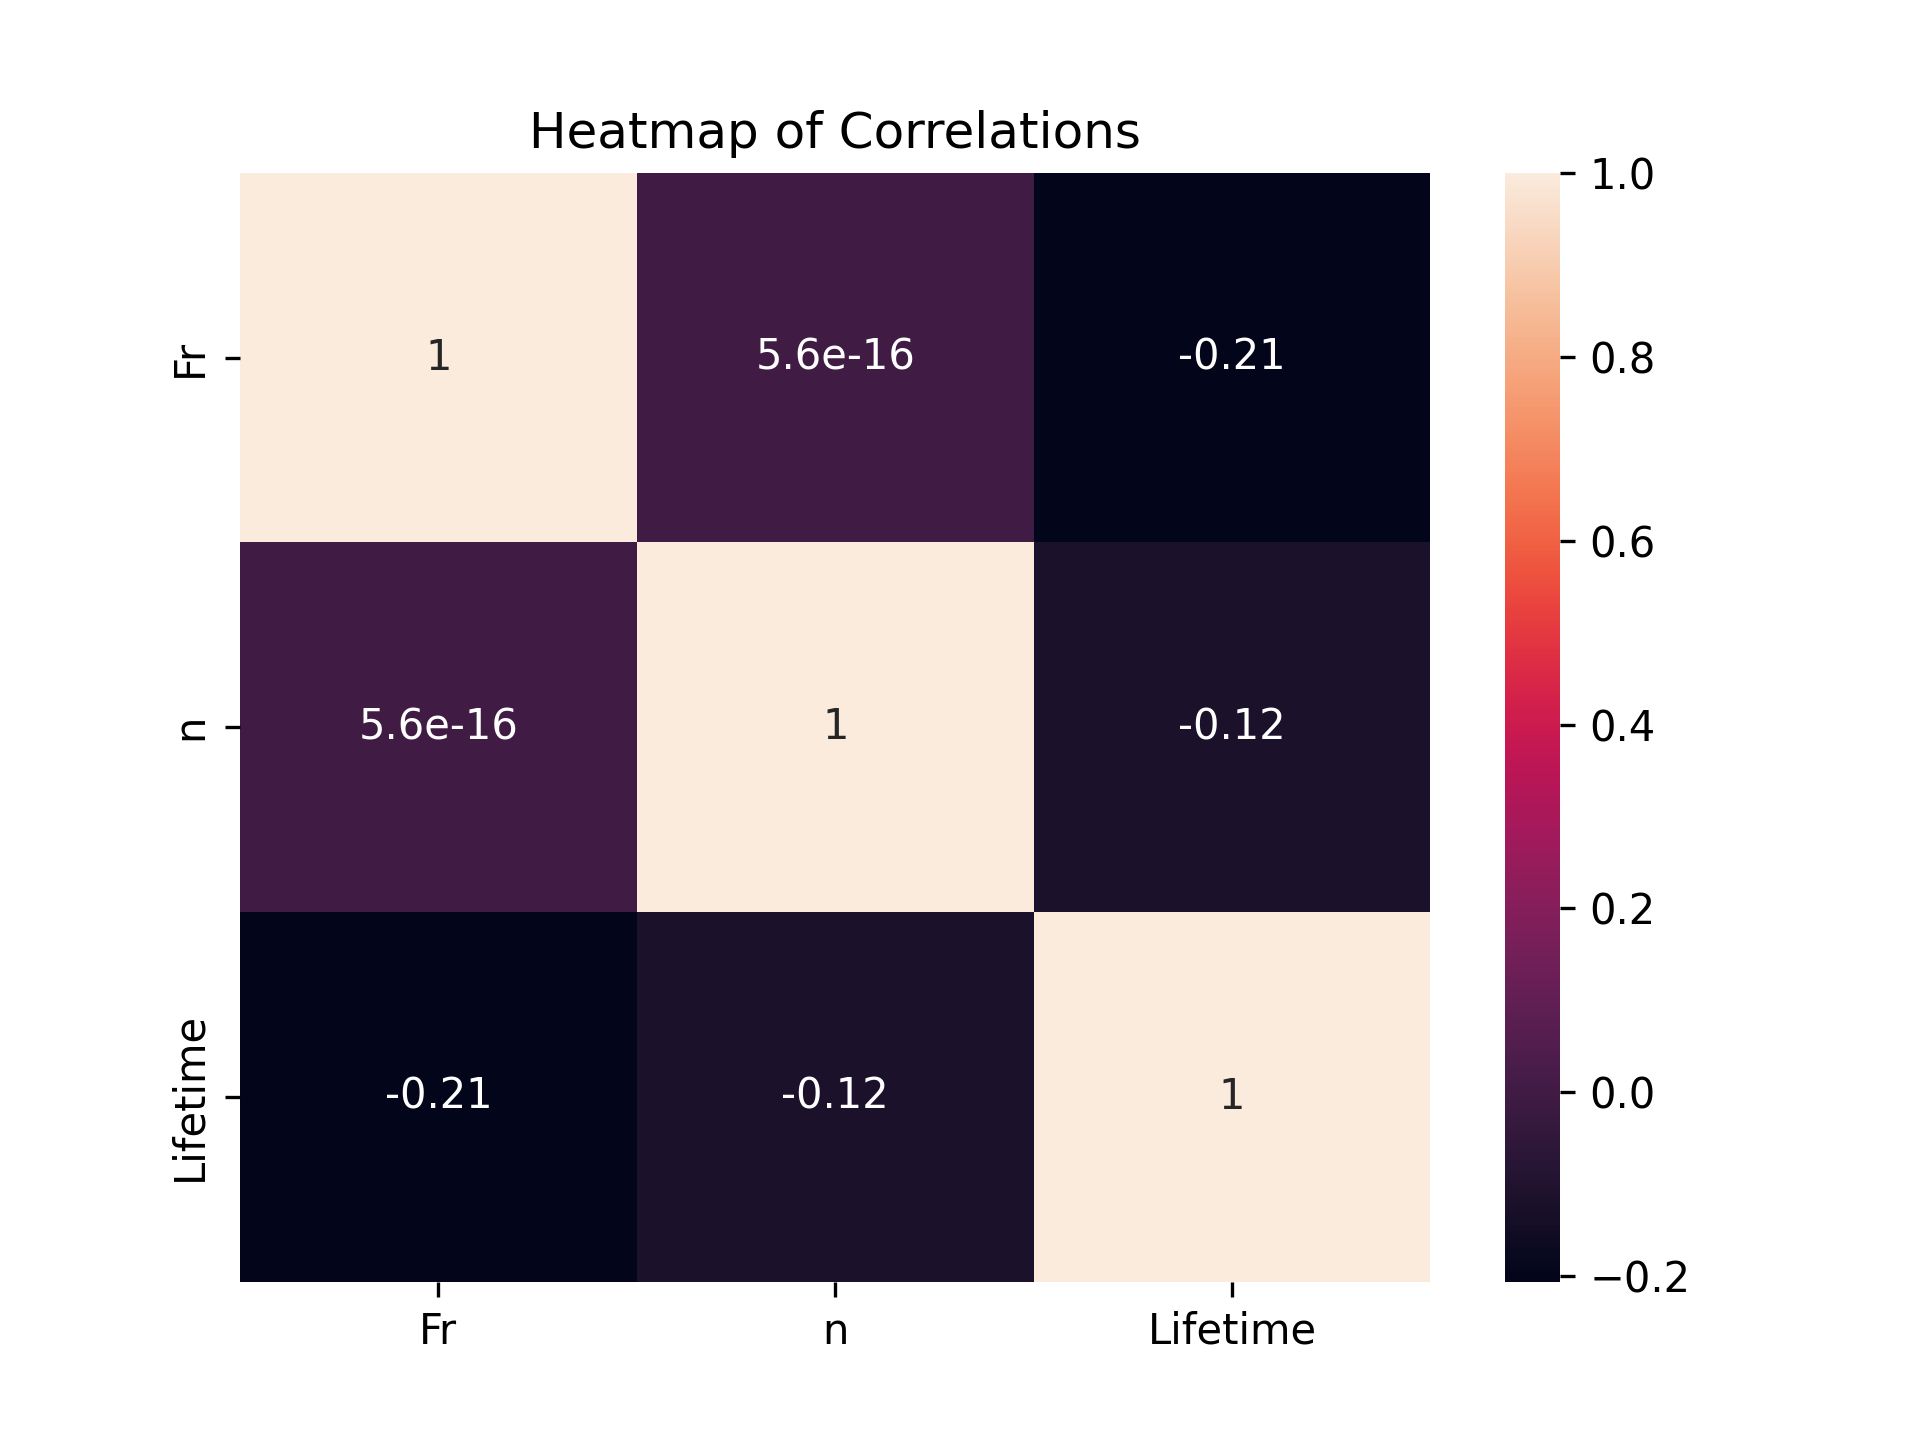
\includegraphics[width=\textwidth]{assets/bearings-eda/correlation-matrix.png}
    \caption{Correlation matrix of variables}
    \label{fig:bearings-corrmat}
\end{figure}

The correlation matrix highlighted an intriguing characteristic of our engineered feature \(Fr/n\). This feature exhibited a distinctive correlation with \(Fr\), indicating a proportional relationship. From this, we could infer the relative weight of the exponents in our potential model equation by examining the inverse of this correlation. This gave us a critical clue towards the development of our hypothesis and shaped our understanding of the relationships within the dataset.

Through multivariate analysis and feature engineering, we've enriched our dataset and gained insights into the relationships between the variables. These findings will now serve as the foundation for the generation of our hypothesis in the next section.


\section{Hypothesis Generation}

During our \ac{eda}, we observed an inverse relationship between \(Lifetime\) and both \(Fr\) and \(n\). This relationship suggested an exponential decay form, as depicted by the 3D plot. From this observation, we hypothesized that the relationship could be represented by a function of the form:

\begin{equation}
\label{eq:hypothesis}
Lifetime \approx c \cdot Fr^{-a} \cdot n^{-b}
\end{equation}

where \(a\) and \(b\) represent the relative influence of \(Fr\) and \(n\) on \(Lifetime\). This exponential function indicates a multiplicative interaction between \(Fr\) and \(n\), each with an inverse relationship with \(Lifetime\). The constant \(c\) scales the function to the correct value range.

To further refine our hypothesis, we performed a sensitivity analysis. By investigating the response of the \(Lifetime\) to a change in the \(Fr\) and \(n\) values, we found that when \(Fr\) doubles, the \(Lifetime\) reduces to approximately \(\frac{1}{10.08}\) of the original. Conversely, when \(n\) doubles, the \(Lifetime\) becomes half. 

Using these observations, we can mathematically derive the weights \(a\) and \(b\). If doubling \(Fr\) (replacing \(Fr\) with \(2Fr\)) results in \(Lifetime\) being roughly one-tenth of the original, it implies that \(2^{-a} = \frac{1}{10.08}\). By solving this equation, we find \(a = -\log_2(\frac{1}{10.08}) \approx \frac{10}{3}\). This value represents the weight of \(Fr\) in our model function.

Similarly, if doubling \(n\) (replacing \(n\) with \(2n\)) results in \(Lifetime\) being half of the original, it implies that \(2^{-b} = 0.5\). Solving this equation, we find \(b = -\log_2(0.5) = 1\).

Using these values for \(a\) and \(b\), we then calculated \(c\) by comparing the actual \(Lifetime\) values with \(Fr^{-a} \cdot n^{-b}\) for the data point with the highest \(Lifetime\). This yielded a constant value for \(c\).

\begin{equation}
\label{eq:constant_c}
c \approx \frac{88445568.46}{200^{-10/3} \cdot 100^{-1}} \approx 4.1378625769 \cdot 10^{17}
\end{equation}

Our refined empirical hypothesis for the function form thus became:

\begin{equation}
\label{eq:refined_hypothesis}
Lifetime \approx \frac{4.1378625767 \cdot 10^{17}}{Fr^{10/3} \cdot n}
\end{equation}

This hypothesis serves as a benchmark and starting point for our model. To assess the fit of our function to the dataset, we calculated the relative error between the \(Lifetime\) and the function's output. The error primarily consists of rounding errors, as our refined formula closely approximates the original dataset.

The relative error was calculated as follows:

\begin{equation}
\text{relative error} = \left(\frac{\text{actual Lifetime}}{\text{predicted Lifetime}}\right) - 1
\end{equation}

This calculation provides a normalized measure of how the predicted Lifetime deviates from the actual Lifetime in the dataset.

The mean of the relative error is \(4.56 \cdot 10^{-12}\), very close to zero, and the standard deviation is \(1.34 \cdot 10^{-10}\), indicating that the error is tightly clustered around the mean. Figure (\ref{fig:bearings-error}) visually supports this, showing the relative error on the z-axis. Despite the plot's limited precision, it's evident that the values represent a very narrow range between \(-4.72 \cdot 10^{-10}\) and \(4.56 \cdot 10^{-10}\).

\begin{figure}[ht]
    \centering
    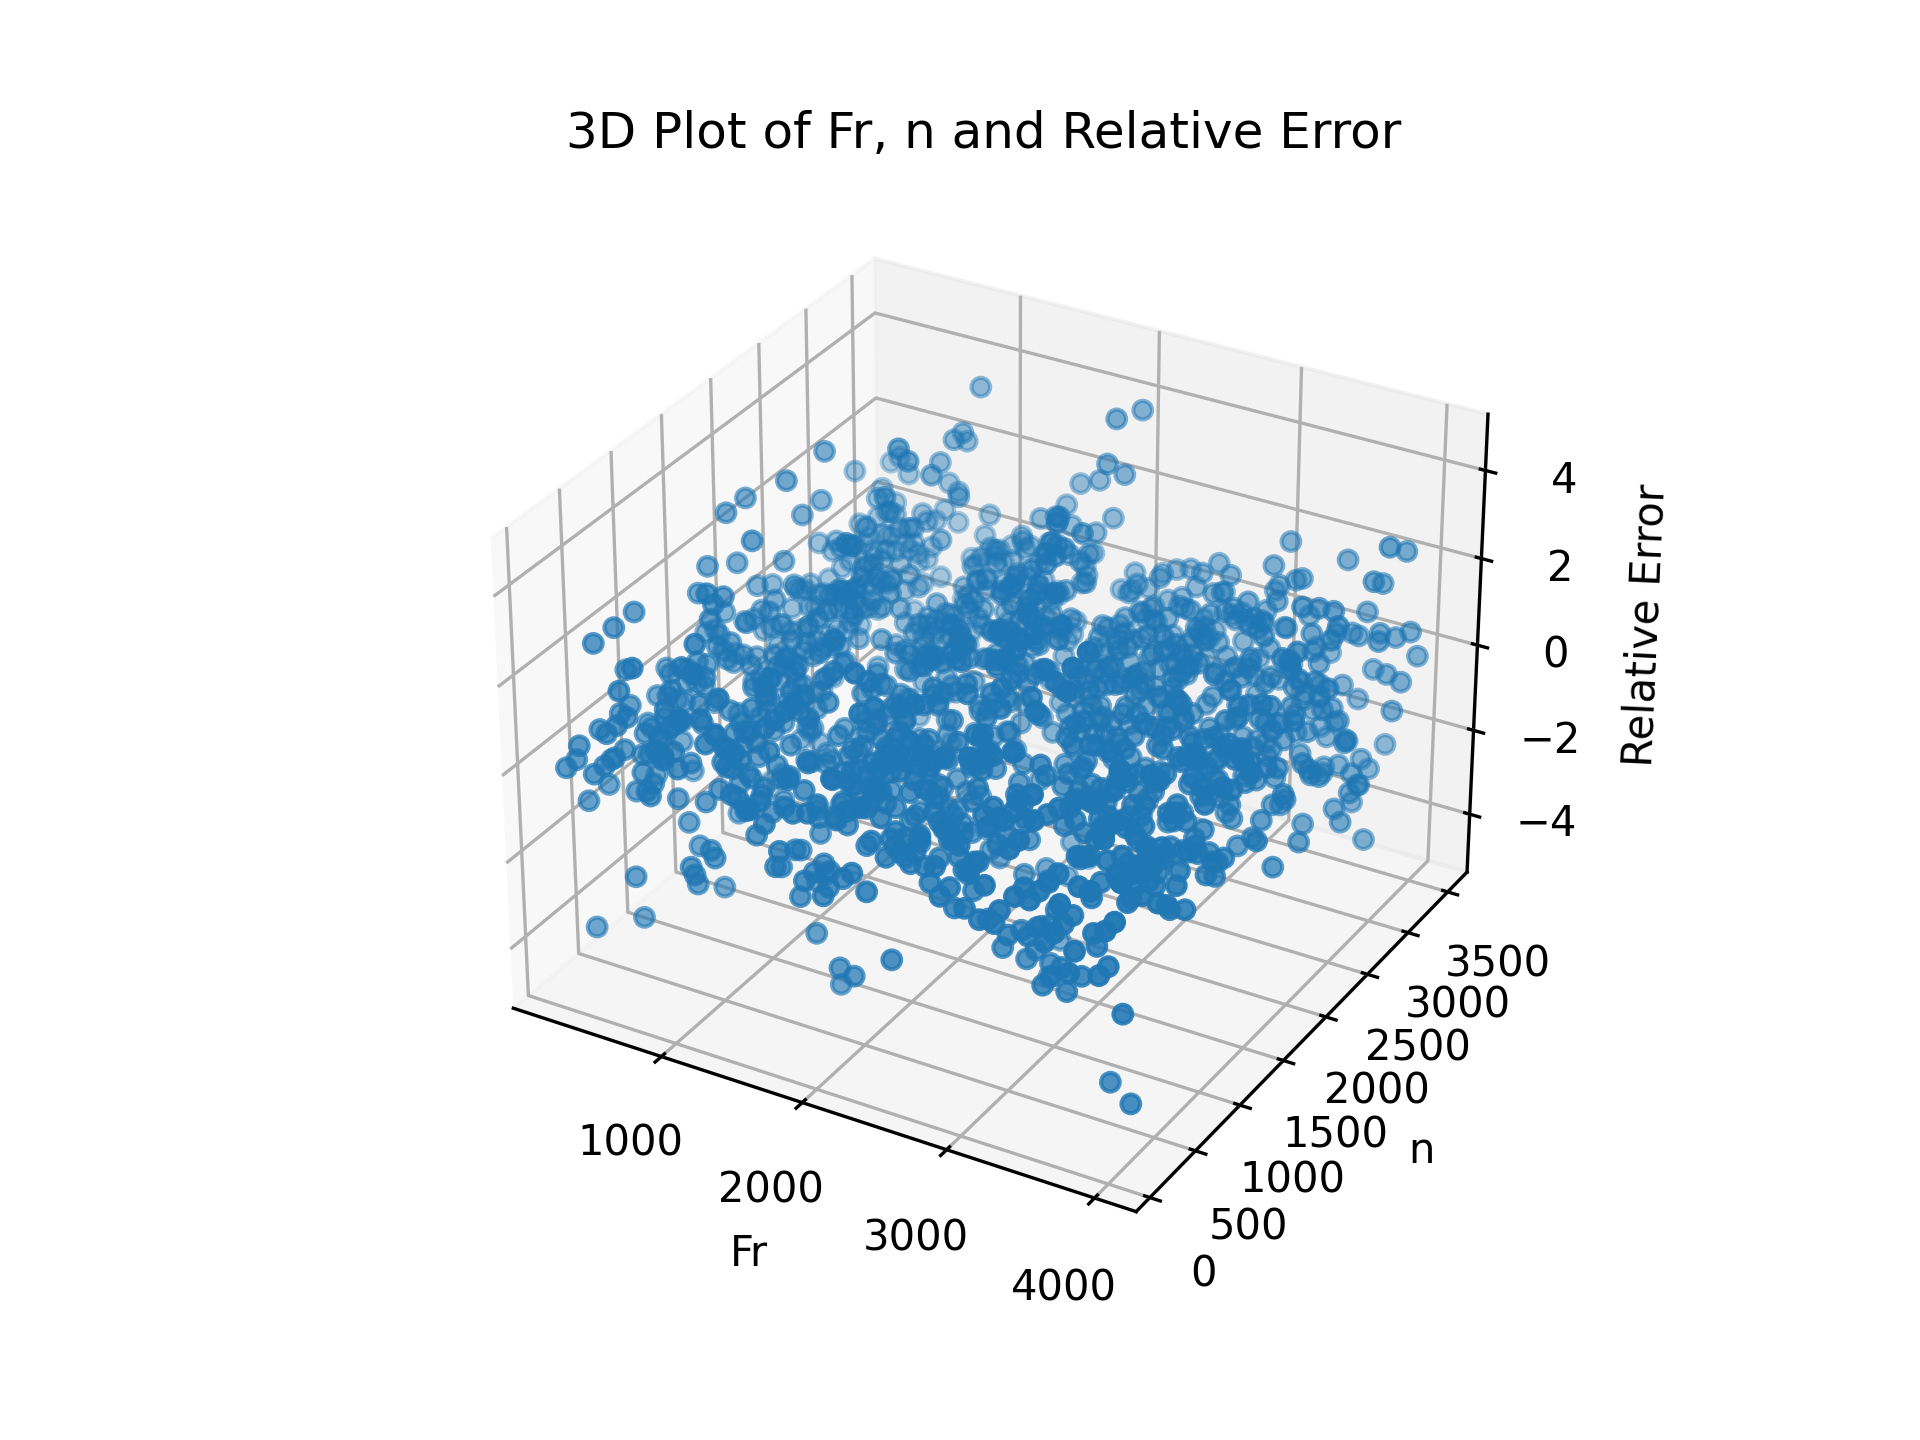
\includegraphics[width=\textwidth]{assets/bearings-eda/3dplot-error.png}
    \caption{3D plot showing the relative error between the actual \(Lifetime\) and the predicted values from our function in \(10^{-10}\).}
    \label{fig:bearings-error}
\end{figure}

The statistical and visual analysis of the relative error confirms that the approximation of the constant \(c\) in our function is highly precise. The minor variations are primarily attributed to the rounding of the \(Lifetime\) values in the dataset. The extreme precision and predictability of the \(Lifetime\) based on \(Fr\) and \(n\) alone suggest that the dataset may have been artificially generated rather than derived from real-world measurements. In practice, other factors would likely introduce more variability and uncertainty into the \(Lifetime\) of the bearings.

Having established this empirical function and assessed its fit to the data, we now have a solid foundation for further modeling. Subsequent stages of our analysis will build on this foundation, making necessary adjustments and improvements to the model.
